\documentclass[10pt]{article} \usepackage[a4paper]{geometry}
\geometry{verbose,tmargin=25mm,bmargin=25mm,lmargin=40mm,rmargin=10mm}
\usepackage{color}
\usepackage{array}
\usepackage{multirow}
\usepackage{amsmath}
\usepackage{setspace}
\usepackage{graphicx}
\usepackage{subfig}
\usepackage{siunitx}
\usepackage{amsmath}
\doublespacing 
\usepackage[pdfusetitle,bookmarks=true,pdfborder={0 0
1},colorlinks=true]{hyperref}
\hypersetup{linkcolor=black,citecolor=black,filecolor=black,urlcolor=black}

\DeclareSIUnit\inch{in}

\usepackage{acronym}

\acrodef{GPU}{Graphics Processing Unit}
\acrodef{CPU}{Central Processing Unit}
\acrodef{SIMD}{Single Instruction Mulitple Data}
\acrodef{GPR}{General Purpose Register}
\acrodef{DLL}{Dynamic Link Library}

\begin{document}

\acresetall

\begin{abstract}
TODO : Abstract
\end{abstract}

\tableofcontents

\acresetall

\cleardoublepage

\section{Introduction}

\section{Literature Review}

\section{Computational Methods}

\subsection{Motion Control}

\subsubsection{Simulator Characteristics}

There are two methods of timing that the system could use:
\begin{itemize}
 \item Fixed time-step - Every simulator cycle is assumed to be a constant 
 length
 \item Variable time-step - The time-step length is proportional to the 
 wall-time elapsed since the last time-step.
\end{itemize}

The real-time length of each time-step was recorded over a period of period of
time.  If a fixed time-step is used, and the simulator is attempting to run in
real-time, the results should show most of the readings at this timestep level,
 with others longer but none singificantly shorter.  A free running real-time
 simulator would display a varying timestep depending on the length of the
 instructions to be executed each cycle, as well as any other activities
 currently taking place on the computer.  This, however, would not be a
 conclusive result, as fixed time-step simulator that isn't running in real-time
 would display similar results.

The distribution produced is shown in figure \ref{fig:timestepDistribution}.  As
 can be seen, the real time-step length varies from
 \SIrange{17.5}{26.0}{\milli\second}, with an approximate normal distribution
 around the mean of \SI{19.17}{\milli\second}.  As discussed previously, it is
 not possible to use this result to determine the simulator's timestep type.
 This could result could equally be a variable time-step length which is being
 effected by other operations on the computer, a real-time fixed time-step
 simulation that is suffering from clock jitter or a fixed time-step simulation
 not running in real-time.

\begin{figure}
 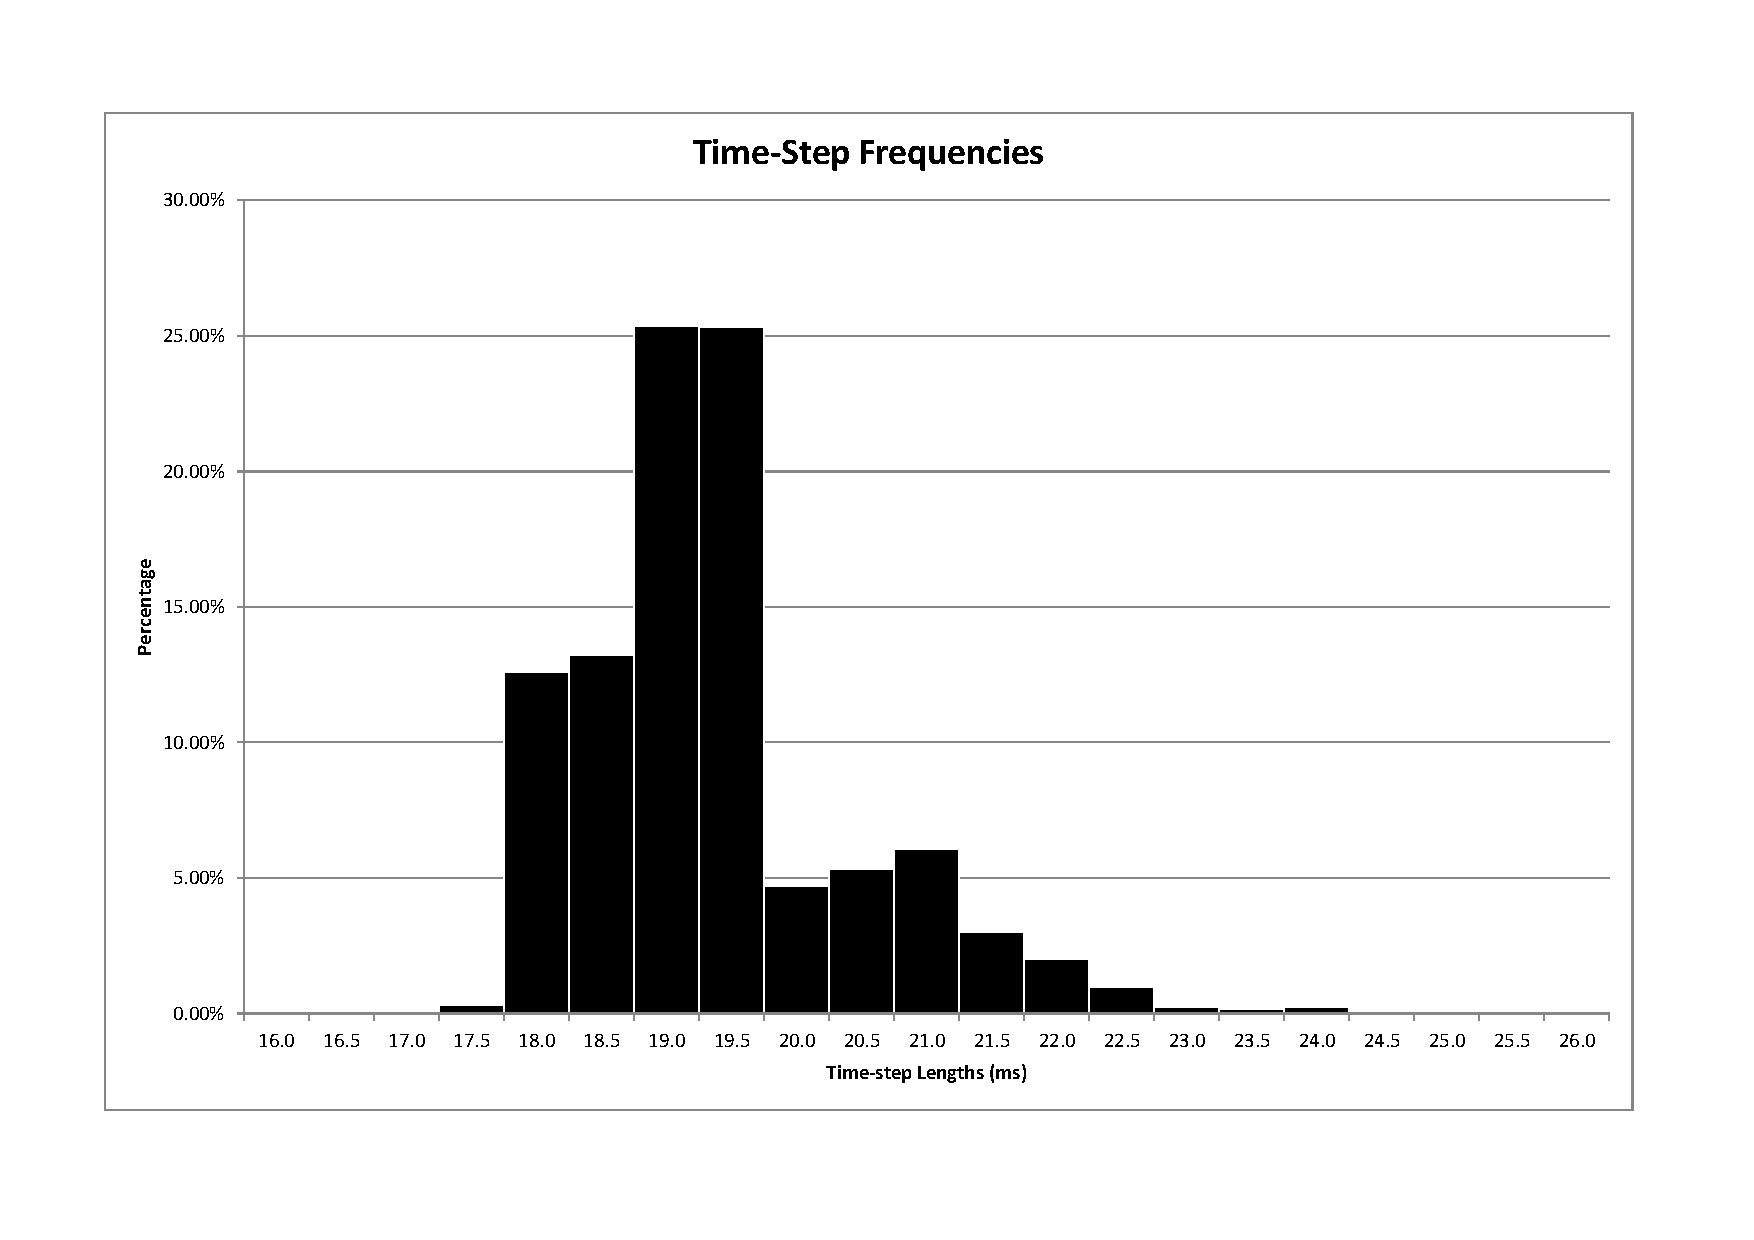
\includegraphics[width=\textwidth]{Images/time-step-length-distribution} \\
 Mean : \SI{19.17}{\milli\second} \\
 Standard Deviation : \SI{1.258}{\milli\second}

 \caption{Time-step Frequency Distribution}
 \label{fig:timestepDistribution}
\end{figure}

An initial run was set up to examine the behaviour of the system over time, and
is shown in figure \ref{fig:initialSpeedTestRun}.  The velocity of the system
(which is determined by dividing the distance travelled by the timestep) has
been calculated with both the measured timestep, as well as a fixed timestep of
\SI{20}{\milli\second} (chosen as a round number approximating the values
measured). The actual value of the fixed time-step is not a concern, as it will
only have a scaling effect on the velocity, which can be accounted for later.

The calculation with a variable timestep (figure
\ref{fig:initialSpeedTestRunVariable}) displays a significant oscilation of the
velocity around the expected behaviour.  In contrast, the fixed time-step values
almost exactly matches the expected behaviour (figure
\ref{fig:initialSpeedTestRunFixed}).  While it is possible that the simulator
could be emulating a non-steady output velocity from the motors, it is expected
that this would display in both graphs.  This makes it very likely that the
time-step used by the simulator has a fixed length.

The anomoly displayed at approximatly \SI{0.6}{\second} on figure
\ref{fig:initialSpeedTestRunFixed} is also seen in a large number of the other
recordings made of this particular scenario.  This is not due to an overly long
simulator cycle length, as this would be hidden by the fixed time-step length. 
The fact that it is present shows that there were one or more simulator cycles
where the system was not updated.  This suggests that it is due to a bug in the
simulator, and any controller will need to be able to handle this sort of error
with minimum disruption.

\begin{figure}
 \centering
 \subfloat[Variable Time-step Length Initial Run
 Velocity]{\label{fig:initialSpeedTestRunVariable}
 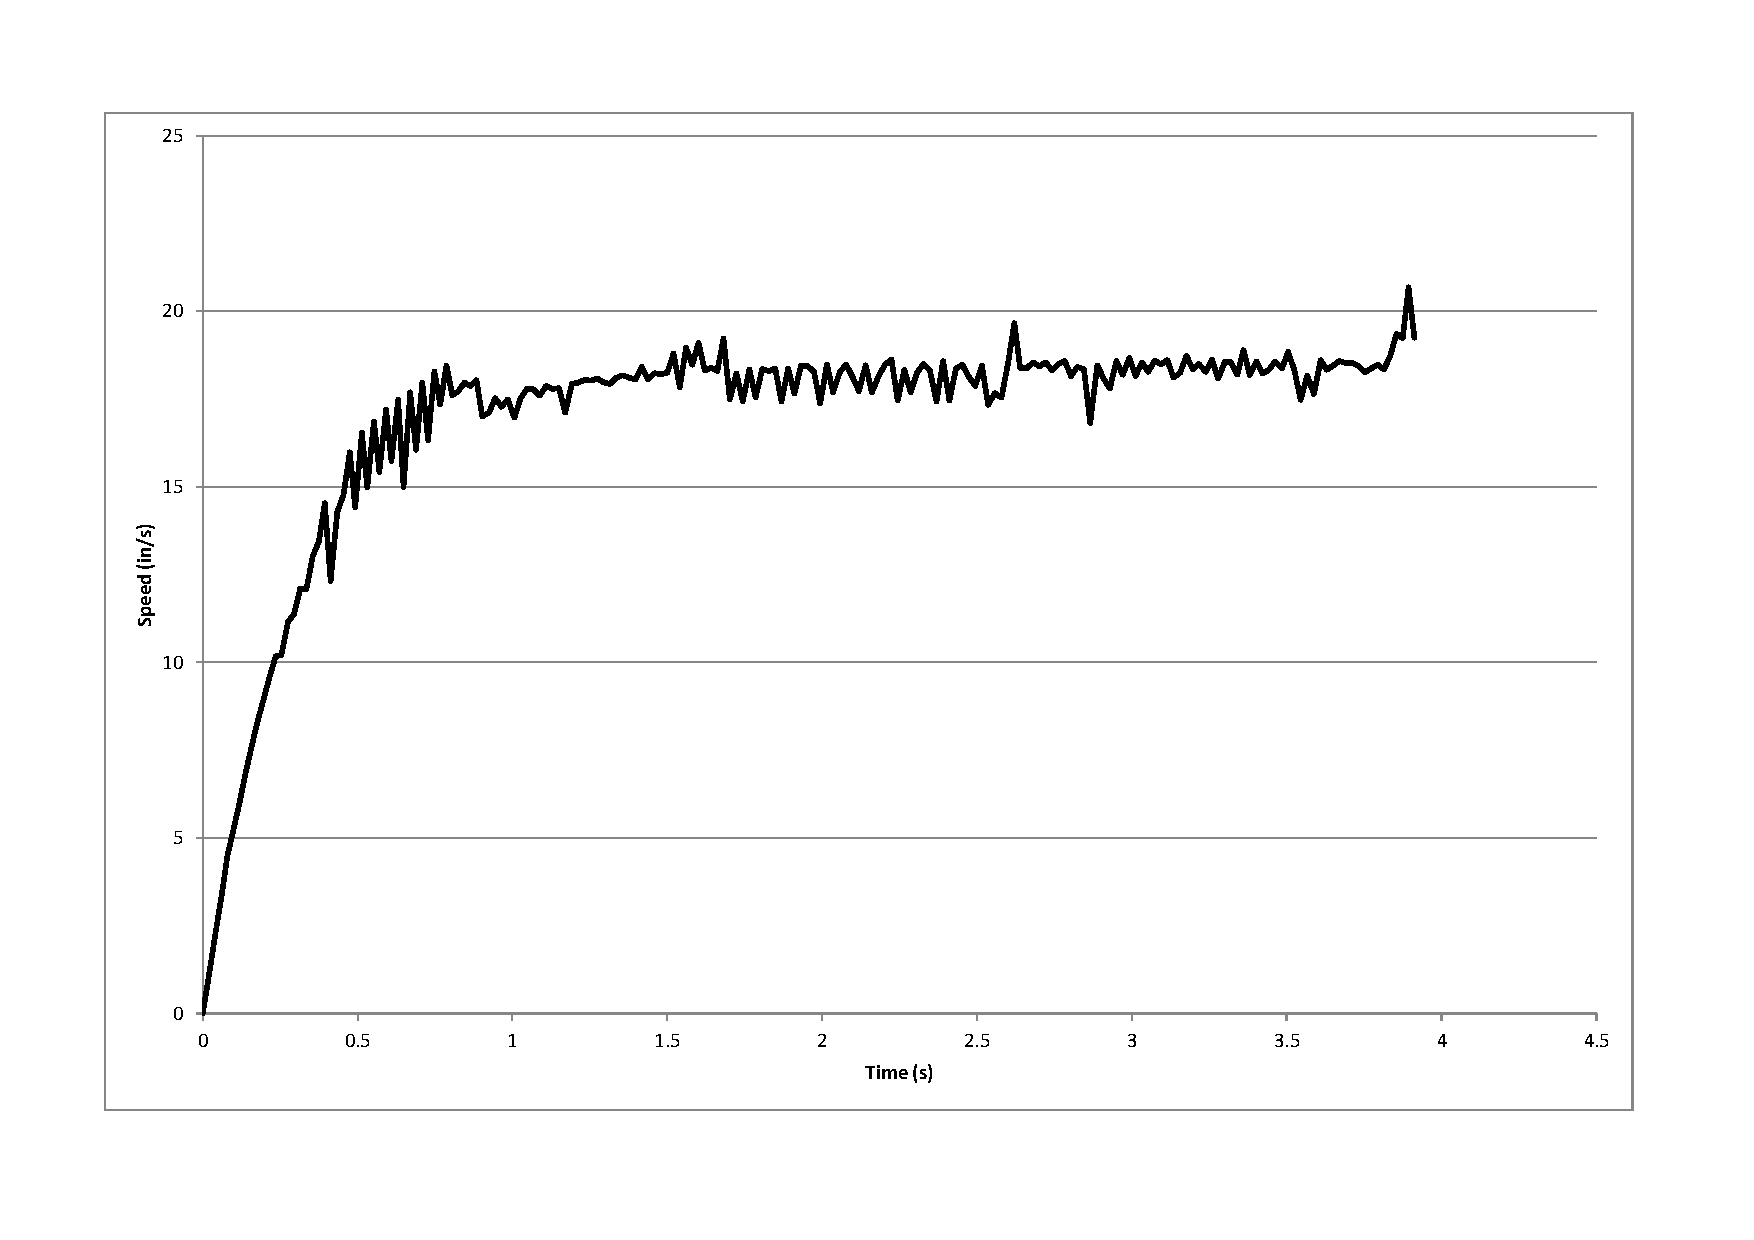
\includegraphics[width=0.8\textwidth]{Images/variable-time-step-initial-run}}
 \\
 \subfloat[Fixed Time-step Length Initial Run
 Velocity]{\label{fig:initialSpeedTestRunFixed}
 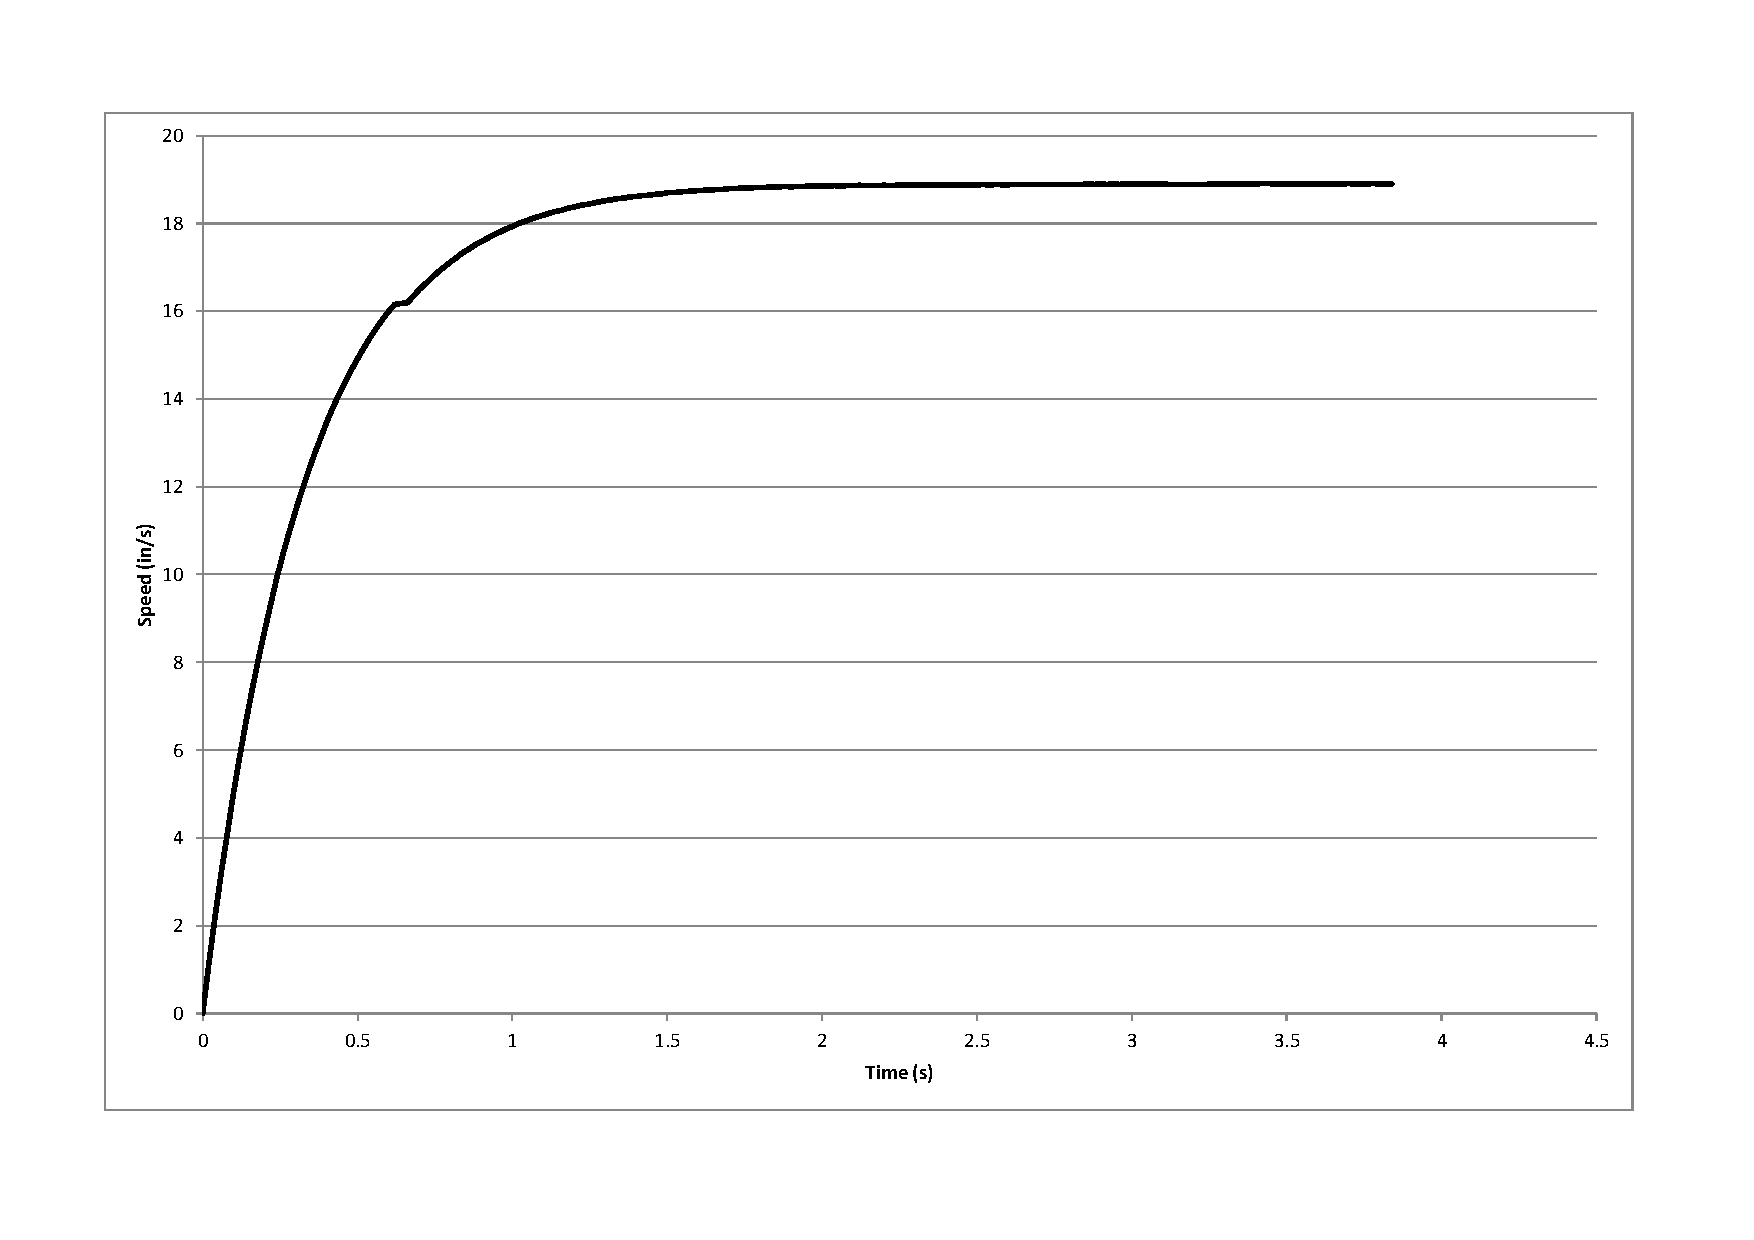
\includegraphics[width=0.8\textwidth]{Images/fixed-time-step-initial-run}}
 \caption{Initial Run Velocities}
 \label{fig:initialSpeedTestRun}
\end{figure}
 
Finally, it was observed that the simulation pauses when the simulator loses the
user focus.  It then resumes without anomaly when the simulator regains the
focus.  As the simulator does not inform this strategies of this, and does not
provide the strategies with any timing data, it is unreasonable to believe that
real-time values are in use.  Were they used, the strategies would experience
control issues caused by the anomalously long time-step if the simulator lost
the focus (and so was suspended) for a significant period of time.  For this
reason, it was assumed that a fixed time-step length was in use, and the length
chosen is \SI{20}{\milli\second}.

\subsubsection{Uncontrolled Behaviour}

The model used for the robots in the simulator is not documented. It is
therefore assumed that the robot's motion is modelled on that produced by an
electric motor. The basic behaviour of the system should be described by the 
transfer function in equation \ref{eq:basicMotorModel} \cite{basicControlNotes}.

\begin{equation}
 \label{eq:basicMotorModel}
 G\left(s\right) = A \cdot \frac{1}{s+B}
\end{equation}

In order to determine the values of the constants $A$ and $B$, a simple strategy
was set up that fed one of the robots a fixed control signal.  This caused it to
accelerate in a straight line until it reached a constant speed.  The position
at each timestep was recorded, to allow the velocity and acceleration to be
calculated.  This was repeated with a number of different input signals, until
the robot could no longer achieve a stead-state speed without colliding with a
wall.

If the model is correct, the steady-state velocity should be directly
proportional to the input velocity.  The steady-state velocity was calculated by
averaging the final ten samples of each simulation, and is plotted against input
signal in figure \ref{fig:inputOutputVelocityGraph}.  A line of best fit has
been plotted to demonstrates the linear relationshi between input and output.

It is interesting to note that the best fit ($R^2 = 1$) is achieved if the
constraint that zero input produces zero output is removed.  This infers that
there is a systematic error that is being introduced by the simulation.  This
will be disregarded in this case, as the error is small
(\SI{-0.3405}{\inch\per\second}) and so should have minimal effect on the
behaviour of the controller.

In order to determine the equation controlling the system, the velocity data was
first normalised by dividing it by the input signal.  This allows the various
volecity profiles recorded to be compared.  The systematic error observed will
cause the data to become slightly distorted, but as previously mentioned, it is
believed the effect will be small.  The MATLAB Curve Fitting Toolbox was then
used to fit the data to a curve.

The best fit achieved is shown in figure \ref{fig:bestFit}.  This is fitting the
data to an equation of the form $y = a \cdot e^{bx} - c \cdot e^{dx} $.  The
function was expected to be of the form $y = a(1-b \cdot e^{cx})$, as this is
what is the form of the time-domain response of the theoretical model in
equation \ref{eq:basicMotorModel} to a step-input.

It was noted that the $b$ term is very small, and the $a$ and $c$ terms are
approximatly the same.  Therefore, it was expected that the model could be
approximated with an equation of the latter form.  This is illustrated in figure
\ref{fig:approximateFit}, which demonstrates an acceptable fit to the majority
of the data.

It was noted that some of the data in the plot appears to be shifted along in
the time-axis, and which is likely interfering with the line fitting process.
This was determined to be due to an error in the original data, where the time
had not been reset to zero at an appropriate point on one of the test runs.
When the data was shifted back into a more expected location, the approximate
fit was improved (shown in figure \ref{fig:approximateFitTimeShiftRemoved}).

Using this information, the system can be modelled with equation
\ref{eq:finalMotorModel}.  This was then used to design the control systems
required.

\begin{equation}
 \label{eq:finalMotorModel}
 G\left(s\right) = \frac{2.12778}{s+2.863}
\end{equation}

\begin{figure}
 \centering
 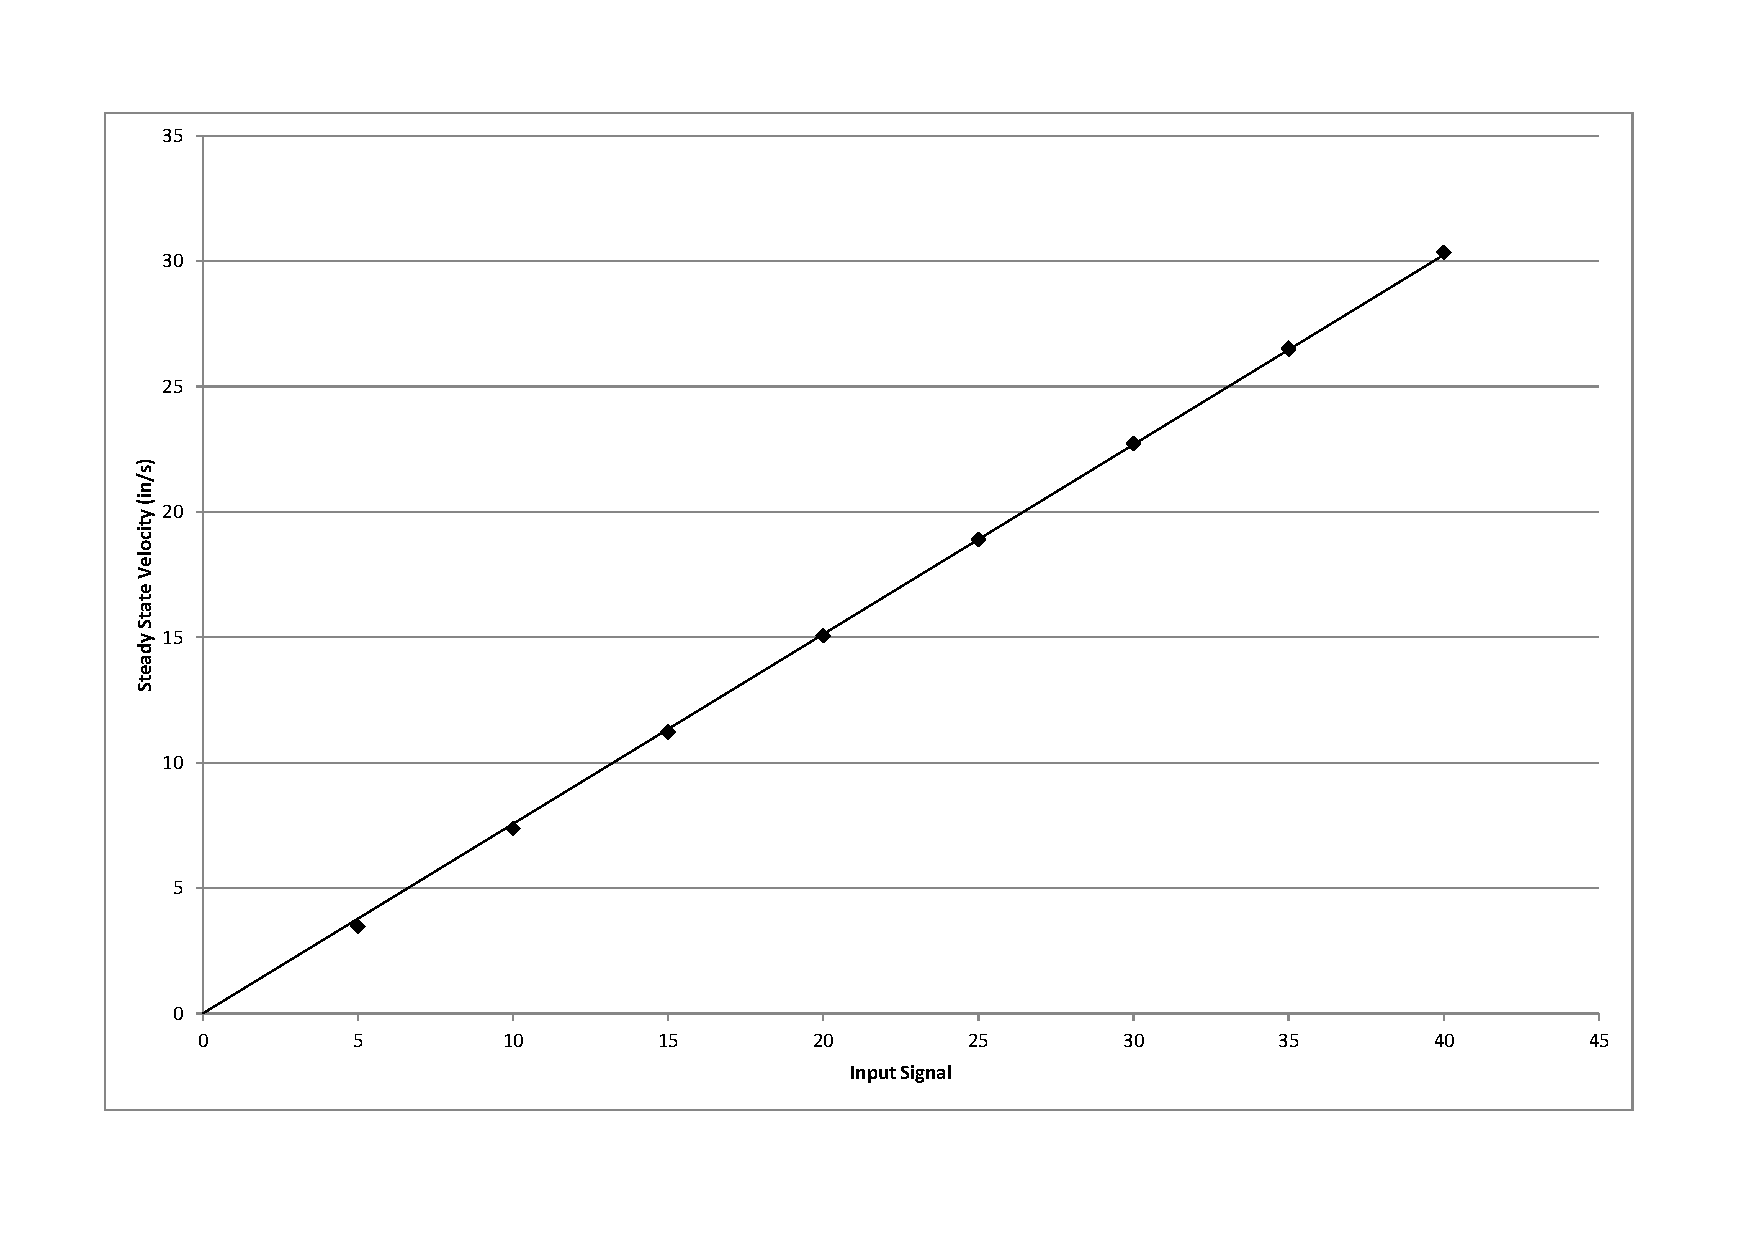
\includegraphics[width=0.8\textwidth]{Images/input-signal-vs-output-speed}
 \caption{Input Control Signal vs Output Velocity}
 \label{fig:inputOutputVelocityGraph}
 
 Line of best fit: $y=0.7564x$ \\
 Quality of fit: $R^2 = 0.9998$
\end{figure}

\begin{figure}
 \centering
 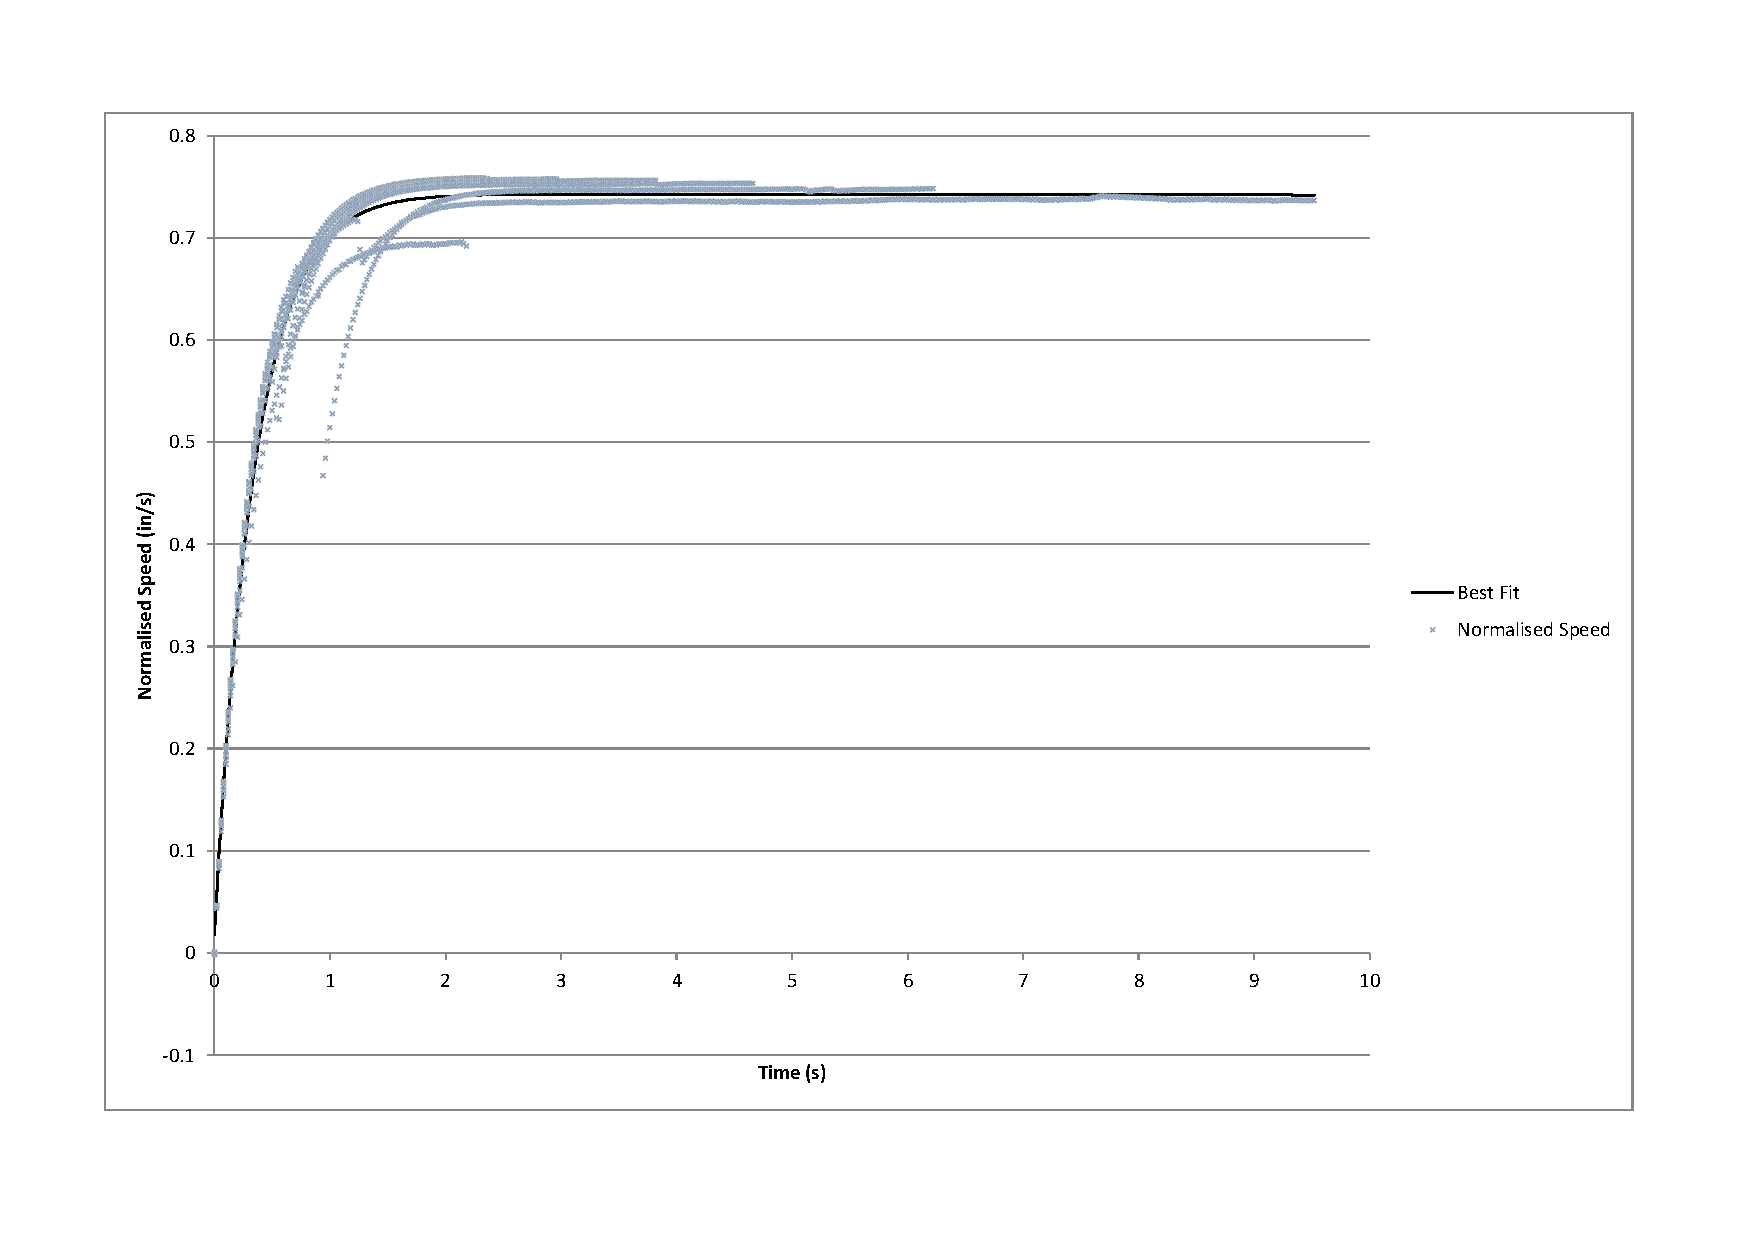
\includegraphics[width=0.8\textwidth]{Images/best-fit-model}
 \caption{Curve Fitting Toolbox Best Fit}
 \label{fig:bestFit}
 
 Line of best fit : $y=0.7432 e^{-0.0001886x}-0.7248 e^{-2.863x}$ \\
 Quality of fit : $R^2 = 0.976$
\end{figure}

\begin{figure}
 \centering
 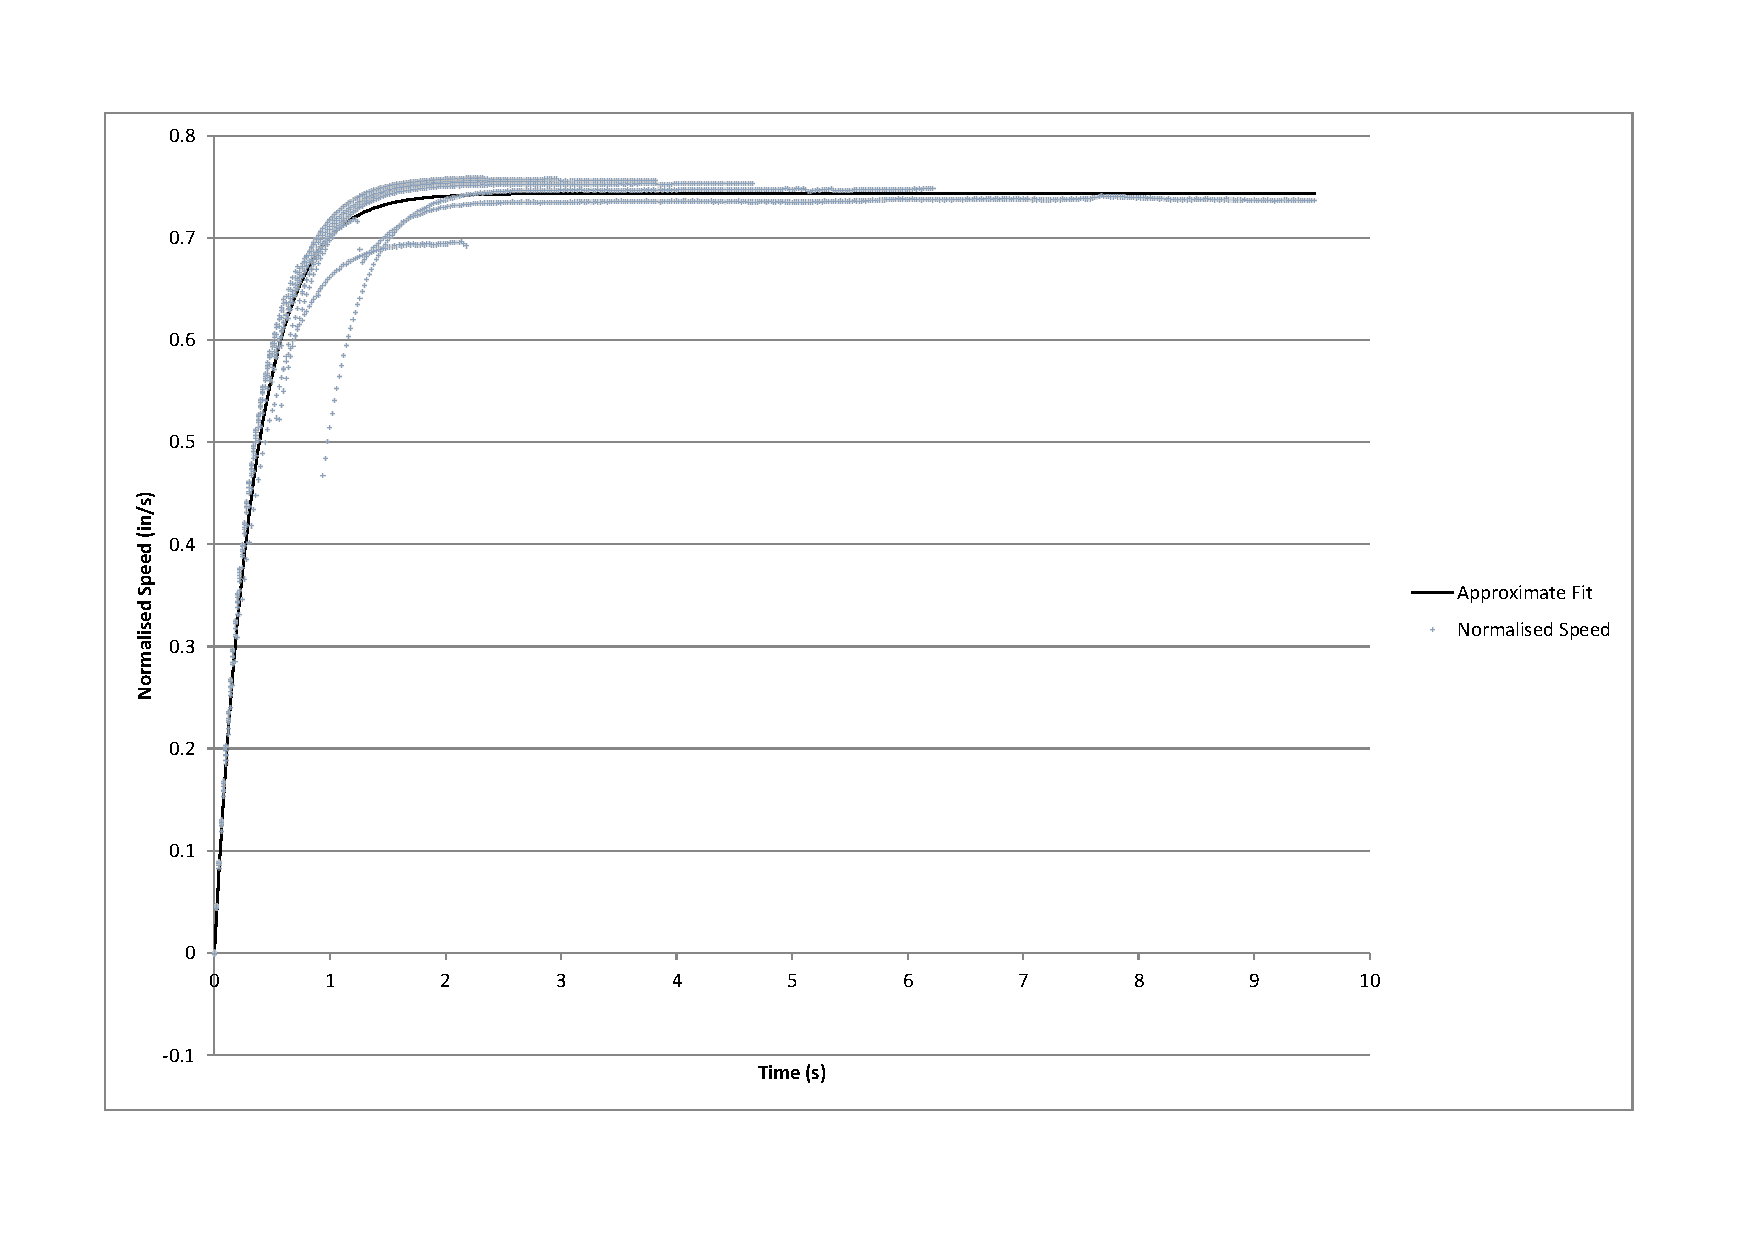
\includegraphics[width=0.8\textwidth]{Images/approximate-fit-model}
 \caption{Approximated Curve Fit}
 \label{fig:approximateFit}
 
 Line of best fit : $y=0.7432 \left(1-e^{-2.863x}\right)$
\end{figure}

\begin{figure}
 \centering
 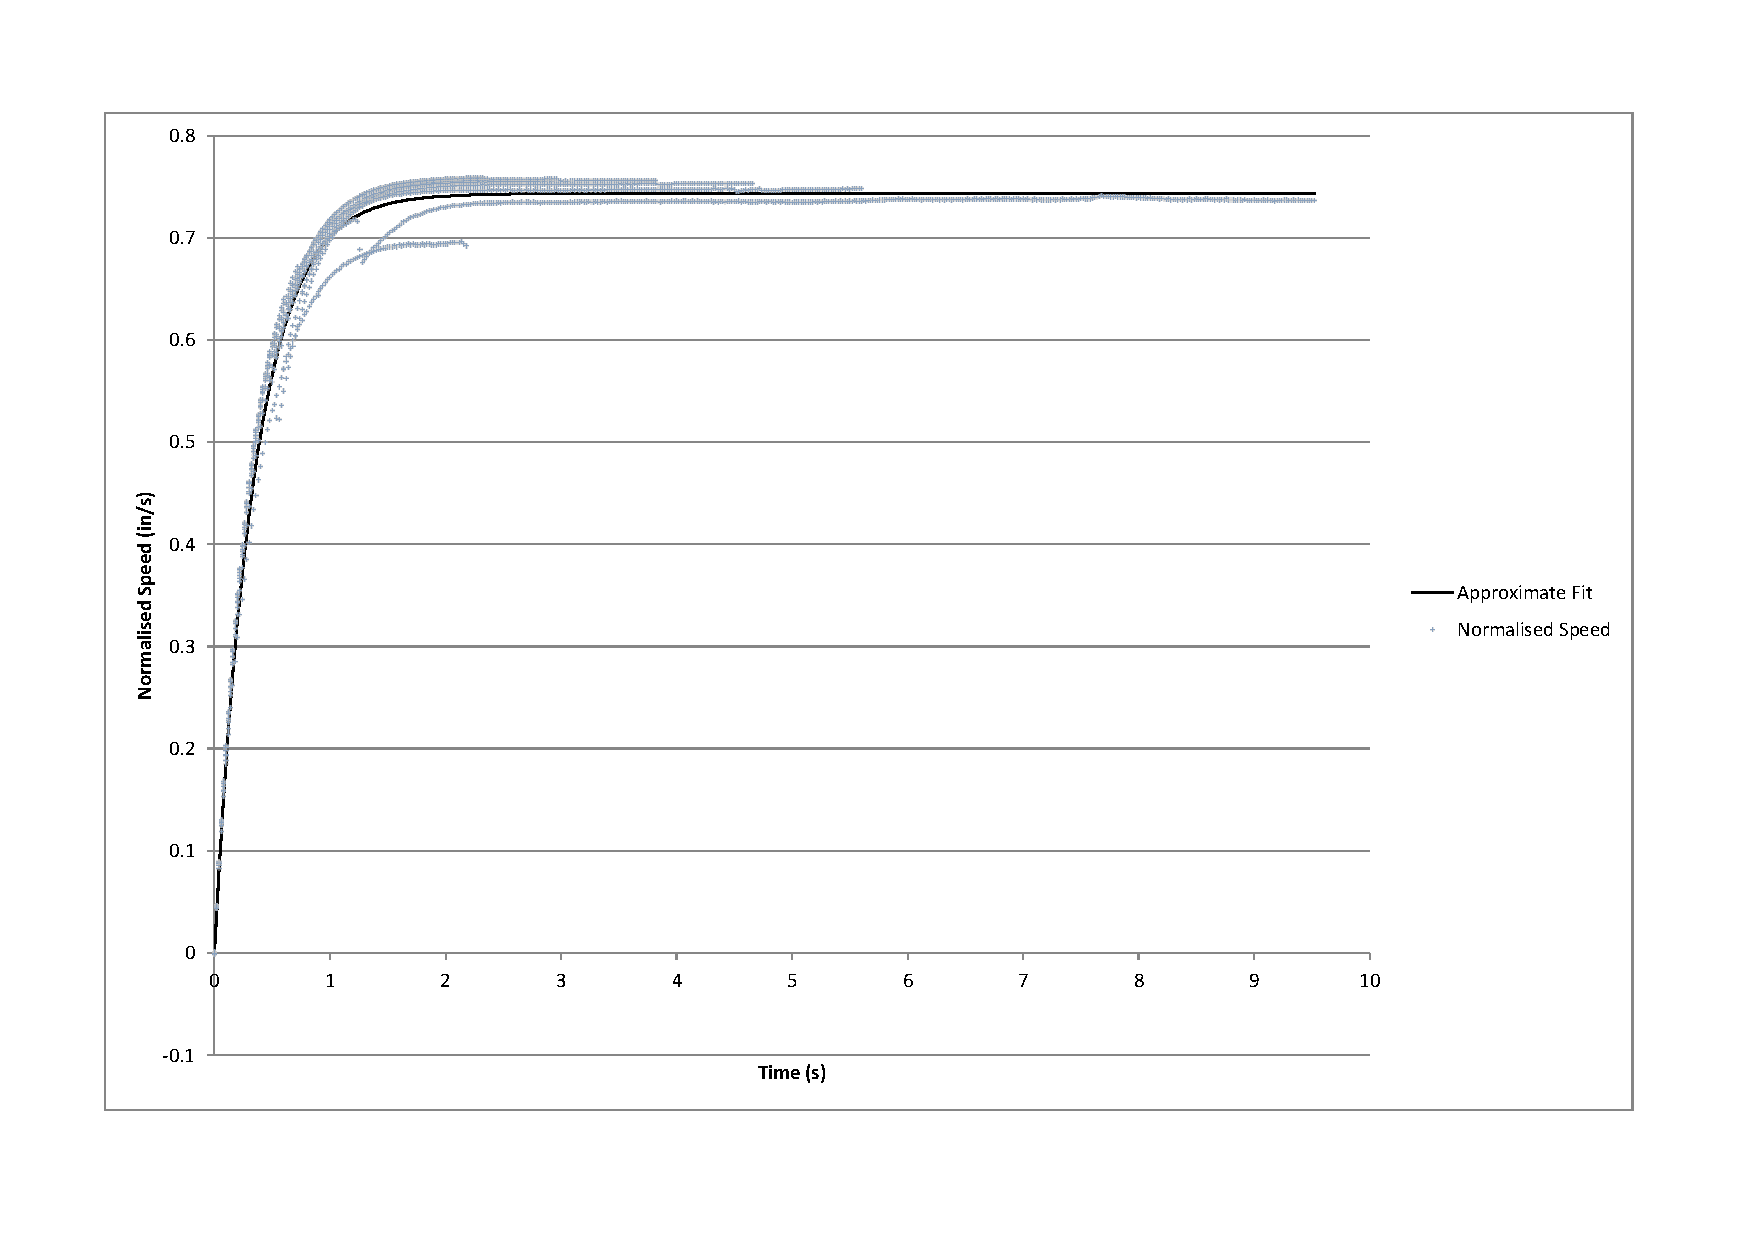
\includegraphics[width=0.8\textwidth]{Images/approximate-fit-model-time-shift}
 \caption{Approximated Curve Fit with Corrected Data}
 \label{fig:approximateFitTimeShiftRemoved}
 
 Line of best fit : $y=0.7432 \left(1-e^{-2.863x}\right)$
\end{figure}

\subsubsection{Controllers}

In order to allow the control of position or velocity desired, the motion
control was implemented using two layers of control.  The first layer controls
the velocity of the robot, while the second layer manipulates the first to
control position.

Both layers are simple proportional controllers, with the velocity control
receiving velocity feedback and the position control receiving position
feedback.  The overall control design is shown in figure
\ref{fig:overalController}.  

The gains were tuned using the MATLAB controller design tools.  The velocity
controller were handled first, to ensure that it would stand alone, and then
motion controller was tuned to adequatly control the resulting velocity.  The
gains calculated were then transferred to the C++ classes VelocityController and
MotionController to be tested.

Unfortunatly, when the code was tested, it was found that the system was highly
unstable, and the specific reasons could not be isolated.  As the aim of the
project was to investigate the high-level control of the robot, rather than the
low-level motor control, the problem was not closely examined.  Instead a set of
gains were produced by a trial-and-error method, which produced a sub-optimal
but stable system.

The control of the angle of motion was achieved by noting the similarity between
the robot footballers and the Mouse robot used in the second year project
\cite{mouseProjectReport}.  The direction of motion was changed by altering the
relative velocities of the individual wheels, which causes the robot to move
through an arc.  Proportional control was again used for this purpose, with the
velocity different proportional to the angular error.

It is recognised that the controllers in use are likely not the optimal designs
that could be used for the system.  While this will have an effect on the
performance of the robot (and so the range of motions that can be performed), it
was decided that investigating the higher level control was more important for
this specific work.  The effect of a better control system can then be
investigated in the future.

\subsection{Potential Field Force Navigation\label{sub:Potential-Field-Force}}

With this technique, a potential field is used to create a force that guides
each robot around the field (as described in
\cite{intelligentAlgorithmPathPlanning}). The field is produced by taking a
collection of objects and projecting a field around them of a given shape. This
field can either add to or subtract from the total field potential surrounding
it. The total field can then be calculated with equation
\ref{eq:fieldSummation}.

\begin{equation}
P(x,y)=\sum_{i=0}^{N-1}p_{i}\left(x,y\right)\label{eq:fieldSummation}
\end{equation}

Where:

$P\left(x,y\right)$ is the total field potential at point $\left(x,y\right)$.

$p_{i}\left(x,y\right)$ is the potential produced by object $i$ at a point.

$N$ is the number of field producing objects.

The direction that the robot will move in is then determined by the gradient of
the field at the current point, such that the robot moves down the field
potential. The force vector (which controls the velocity of the robot) is given
by equation \ref{eq:forceSummation}.

\begin{equation}
\boldsymbol{F}(x,y)=-\left(\frac{{\partial P\left(x,y\right)}}{\partial x}+\frac{{\partial P\left(x,y\right)}}{\partial y}j\right)\label{eq:forceSummation}
\end{equation}

If the fields can be differentiated over the entire field, this can be
calculated as in equation \ref{eq:forceDifferentiation}.

\begin{equation}
\boldsymbol{F}(x,y)=-\left(\sum_{i=0}^{N-1}\frac{\partial p_{i}\left(x,y\right)}{\partial x}+\frac{\partial p_{i}\left(x,y\right)}{\partial y}j\right)\label{eq:forceDifferentiation}
\end{equation}

However, if one or more of the fields cannot be differentiated, the force vector
must be calculated discretely. This is achieved using equation .

\begin{equation}
\boldsymbol{F}(x,y)=\left(P\left(x-1,y\right)-P\left(x+1,y\right)\right)+\left(P\left(x,y-1\right)-P\left(x,y+1\right)\right)j
\end{equation}

The negative gradient is used to ensure the robot moves towards lower field
potentials. The technique would work equally well if it was attracted to higher
field potentials, provided all the equations were suitably inverted.

For the initial control technique, the velocity of the robot is proportional to
the force vector. Other techniques are discussed by
\cite{intelligentAlgorithmPathPlanning}, but will be experimented on later.

Navigation of the game field can now be achieved by manipulating the attractive
and repulsive fields to guide the robot to a target. Computational power
allowing, each robot would have a separate field that guides it based on the
goals specific to its role.

\subsection{Potential Field Shapes}

Attractive fields are used to designate areas which the robot should be headed
for. In order to ensure that the robot always heads towards them, it is
important that their effect is felt across the entire field. However, they must
not be so strong that they overwhelm the short distance effects of the repulsive
fields, but strong enough to govern the robot's overall destination.

Repulsive fields are used to alter the route of the robot when heading for these
targets. For example, such fields are used to get the robot to avoid collisions,
as well as to control where the robot intercepts the ball. These fields
typically only act over a short distance, as they should only have an effect
when they are required. They need to be strong enough to overwhelm the
attractive fields at short range.

The field shapes experimented with are described in the following sections, in
order to determine the best combination for each scenario. As the basic fields
in use are axisymmetric in shape (or begin that way), the fields are best
described using polar coordinates. The coordinates are defined as in figure
\ref{fig:polarCoordinateFrame}, and are always centred on the field producing
object. This frame of reference can then be translated to the Cartesian
coordinates in use elsewhere to allow the total field at a point to be
calculated.

\subsubsection{Basic Attractive Field\label{sub:Basic-Attractive-Field}}

The field suggested by \cite{intelligentAlgorithmPathPlanning} for the
attractive point is described with equation \ref{eq:quadraticBallField}.

\begin{equation}
P(r,\theta)=\frac{1}{2}k_{attr}r^{2}\label{eq:quadraticBallField}
\end{equation}

Where $k_{attr}$ is the attractive weight assigned to the ball.

This produces an attractive force that is linearly proportional to the distance
to the object (in this case the ball). This is a very useful field for a route
finder (as described in the paper), where it is desirable for the the robot to
stop when it reaches the destination, and so it needs to slow down as it
approaches the target. However, in this application it is more useful for the
robot to make a rapid approach and not slow down after arrival, as this will hit
the ball away from the robot.

In order to overcome this problem, the field was simplified to equation
\ref{eq:conicBallField}.

\begin{equation}
P(r,\theta)=\frac{1}{2}k_{attr}r\label{eq:conicBallField}
\end{equation}

This field produces a constant force of $k_{attr}$ acting towards the centre of
the ball, which will hold the robot against the ball (as far as possible) as the
ball and robot move around. It doesn't provide any guidance once the ball has
been reached, and so this will need to be provided by an additional field once
the intercept is complete.

\subsubsection{Basic Repulsive Field\label{sub:Basic-Repulsive-Field}}

One of the rules of the game is that the robot cannot intentionally collide with
an opposing robot, unless they are in possession of the ball
\cite{simurosotSim}. This means that the robot must actively avoid the other
robots. It is also advantageous to be able to avoid the robots own team, as this
prevents the robots getting into a position where they cannot move as they are
fighting against each other.

A apparently simple solution would be to surround all the obstacles with a
region of potential that is substantially higher than the surrounding area, as
described by equation \ref{eq:circleRepulseField}.

\begin{equation}
P\left(r,\theta\right)=\begin{cases}
k_{repulse} & r<R_{0}\\
0 & r\geq R_{0}
\end{cases}\label{eq:circleRepulseField}
\end{equation}

Where $k_{repulse}$is the repulsive potential and $R_{0}$is the radius of the
circle. This produces a field as illustrated in figure \ref{fig:circleField}.

In theory, the robot would avoid this circle, as the algorithm should not have
the robot move into a region of high potential. However, this does not work, as
the controller actually responds to the gradient of the field (shown in figure
\ref{fig:circleFieldGradient}). As shown in the figure, this type of field
produces very high force, but only in a very small region. Once inside the
repulsive circle, the gradient returns again to zero, and so does not effect the
motion of the robot. As the robot has inertia, it is very likely that it pass
through the region of high force and then leave it before it's velocity has
altered sufficiently to avoid the obstacle.

In order to maximise the repulsive effect of the field, the force must be
exerted over a large area. This can be achieved with a field that gradually
builds in strength as it nears the obstacle. The simplest example is defined by
equation .

\[
P\left(r,\theta\right)=\begin{cases}
k_{repulse}\cdot r & r<R_{0}\\
0 & r\geq R_{0}
\end{cases}
\]

This field will create a constant force that acts radially away from the
obstacle, much like the attractive force described in section
\ref{sub:Basic-Attractive-Field}, but over a restricted area (as illustrated in
figure \ref{fig:conicRepelField} and \ref{fig:ConicRepelFieldGradient}). If the
target is behind the obstacle, and the force is exactly strong enough, it will
cause the robot to stop in the repulsive field. If the force is too small, it
will only slow the robot down, and if the force is too strong it will cause the
robot to move clear of the field. If the target hasn't moved significantly, the
robot will then approach the repulsive field again, only to be repelled once
more. This will result in the robot repeatedly 'bouncing' off of the field. The
robot will become stuck if the target does not move, but it is thought that the
rapidly changing environment the controller will be working in will mean that
this is not a significant issue.

While the constant force will work, provided it is strong enough, the case when
it is too strong and causes 'bouncing' is undesirable as the motion of the robot
will become erratic. A better solution would be one where the force gradually
increases as it approaches the target. It is also desirable to have a field that
naturally decays to a small level at a distance without relying on conditional
operations. Two field shapes which meet this specification are a direct inverse
proportionality, or the Gaussian function (described by equations
\ref{eq:inverseRepulseField} and \ref{eq:gaussianRepulseField} respectively).

\begin{equation}
P\left(r,\theta\right)=\frac{k_{repulse}}{r}\label{eq:inverseRepulseField}
\end{equation}

\begin{equation}
P\left(r,\theta\right)=k_{repulse}\cdot e^{\left(\frac{r^{2}}{2\sigma_{repulse}}\right)}\label{eq:gaussianRepulseField}
\end{equation}

Where $\sigma_{repulse}$ controls the width of the field.

For this purpose, the Gaussian function was selected, because it was initially
believed that a flatter region in the centre of the field would be preferable
over an infinite field potential (see section TODO). This produces a field as
shown in figure \ref{fig:gaussianField}. As the gradient image shows, this
produces a region of rapidly increasing force around the object, with no
discontinuities that produce disruptive motion at the edge of the field.

\subsubsection{Shaped Approach Guiding Field\label{sub:Shaped-Approach-Guiding}}

As the robot has no means of holding on to the ball, it is not possible for the
robots to turn more than a small amount when in possession of the ball without
losing it. This makes it particularly important that the robot approaches the
ball from the correct side. This can be achieved by positioning a region around
the ball that guides the robot to the correct position.

The initial attempt at this placed a specially shaped field around the ball,
which was developed by rotating a Gaussian function along a circle around the
ball, with it's height proportional to the angle from the desired access
direction. This is described by the equation \ref{eq:wrappedGaussian} and shown
in figure \ref{fig:wrappedGaussianField}.

\begin{equation}
P\left(r,\theta\right)=e^{\frac{-\left(r-r_{0}\right)^{2}}{2\sigma_{repulse}}}\cdot\left|\frac{\theta}{\pi}\right|\label{eq:wrappedGaussian}
\end{equation}

\[
-\pi\leq\theta\leq\pi
\]

This field initially looked promising, as it contains the desired slope towards
a specific approach angle and repels away from every other angle. On testing,
however, it was noticed that, because the field is at a higher potential than
it's surroundings, the edges of the field force the robot radially away from the
ball instead of towards the target angle, and so the robot just stops at the
edge of the field.

The field was then modified to be at a lower potential than it's surroundings,
as shown in equation \ref{eq:insetWrappedGaussian}.

\begin{equation}
P\left(r,\theta\right)=e^{\frac{-\left(r-r_{0}\right)^{2}}{2\sigma_{repulse}}}\cdot\left|\frac{\pi-\theta}{\pi}\right|\label{eq:insetWrappedGaussian}
\end{equation}

This removed the previous radial force. However, it was determined that a field
wide enough to be of any use in directing the robot had to have a radius that
caused the field to strongly interfere with motion elsewhere in the playing
field. When other robots were introduced into the field, even in their starting
positions, the robot was unable to approach the ball without a collision with
another player.

Other attempts were made with different shaped fields around the ball (for
example one field resembled a helter-skelter slide, which produced a constant
force to guide the ball in when within a certain radial region), but all
resulted in either an large field that caused too much long-distance
interference, or forced the robot radially away from the robot. While a field
could probably be found that achieved what was desired, it was determined that
the search would be too time-consuming with the lack of guiding information.

\subsubsection{Paired Source Approach Guidance Field}

As discussed in section \ref{sub:Shaped-Approach-Guiding}, a field was required
to guide robot's the approach to ball. As a single field did not function as
desired, it was decided that a pair of fields would be used.

A basic attractive field (see section \ref{sub:Basic-Attractive-Field}) was
positioned on the desired approach side of the ball (offset by a number of
inches in the $x$ axis) and a basic repulsive field (see section
\ref{sub:Basic-Repulsive-Field}) was placed in the symmetrically opposite
position. This produces the overall field shown in figure
\ref{fig:pairedApproachField}.

This technique immediatly showed positive results, with the robot moving onto
the attractive point while avoiding the ball if it approached from the wrong
side. This is achieved because the combination of the field produces a region
that the robot will not pass through, because to do so would involve passing
through the repulsive region (as shown in figure
\ref{fig:pairedSourceApproachFieldNoFlyZone}).  This field configuration breaks
down if the repulsive point is too far from the ball or if the robot ends up too
near the ball on the wrong side (the region shown in figure
\ref{fig:pairedSourceApproachFieldBreakDownZone}), as the repulsive field acts
to force the robot towards the ball instead of away from it.  The strategy will
need to be designed so that this occurence is dealt with, or prevented from
happening altogher.

To ensure that the robot approaches from the correct location, the points must
be placed to position the robot along the line that joins the ball and the
desired desination (initially, the goal).  This is achieved by providing this
vector to the field calculation code, which then sets the point locations
appropriately.

TODO : Consider including a video showing this in action, or perhaps include it
in the results section.

When this field is in use, the robot is not attracted to the actual position of
the ball, and so this field will not allow the robot to guide it to the goal.
However, if a new set of field configurations are used once this robot is in
position, this limitation can be overcome.

\subsection{Field Calculations}

In order to determine the direction the robot should move in, the field needs to
be calculated at four points, as described in section
\ref{sub:Potential-Field-Force}. Even for the most complex fields in use, this
is not particularly computationally challenging. However, the efficiency of the
code could be improved by vectorising the data and taking advantage of the
\ac{SIMD} instructions available on most modern \acp{CPU} to calculate all four
points simultaneously. This would allow the field calculations to take less
time, resulting in more time available per time-step to perform other
operations.

In addition, it is useful to render the entire field as an image, so that it can
be considered for debugging purposes. Given that the playing field is
approximately \SI{88}{\inch} by \SI{72}{\inch}, and is being considered at
\SI[quotient-mode = fraction]{1 / 10}{\inch} scale, this gives \num{633600} data
points to consider. This size of dataset will require a large amount of \ac{CPU}
cycles to calculate, even if the individual data point's requirements are
relatively modest. With further delays introduced by inter-process communication
(it is not possible to alter the simulator to produce the image locally), as
well as other delays and overheads introduced by the operating system, it
quickly becomes challenging to render the field in real-time.

The calculation times for both the entire field and a set of four points using
the OpenCl code on both the \ac{CPU} and \ac{GPU} are shown in table
\ref{tab:Field-Strenth-Calculation}. These clearly show that the calculation of
the entire field is best done on the GPU, where the acceleration from the
massively parallel computation structure masks the additional overheads. The
four points, however, are best done on the \ac{CPU}, where it does not suffer
from the significantly larger memory transfer times which affect \ac{GPU}
operations.

\begin{singlespace}
\begin{table}
\centering%
\begin{tabular}{|c|m{2cm}|p{2cm}|p{3cm}|m{2cm}|}
\hline
\multirow{2}{*}{Task} & \multirow{2}{3cm}{Computation Platform} &
\multirow{2}{2cm}{Execution Time (\si{\micro\second})} &
\multirow{2}{3cm}{Memory Transfer Time (\si{\micro\second})} & \multirow{2}{2cm}{Total Time (\si{\micro\second})} \\
 &  &  &  & \\
\hline
\multirow{2}{*}{Entire field} & \ac{CPU} & \num{23500} & \num{479} & \num{24100}
\\
\cline{2-5}
 & \ac{GPU} & \num{2050} & \num{2600} & \num{8611} \\
\hline
\multirow{2}{*}{Four data points} & \ac{CPU} & \num{14.4} & \num{0.342} &
\num{60.0}
\\
\cline{2-5}
 & \ac{GPU} & \num{18.8} & \num{1040} & \num{4390} \\
\hline
\end{tabular}

In this test, overheads include transfering the inital data to the platform and
setting up the platform before the calculation, but not one-time-only
intialisation done by the platform.

\caption{Field Strenth Calculation Times\label{tab:Field-Strenth-Calculation}}
\end{table}

\end{singlespace}

\subsubsection{Design Philosophy}

The code (shown in appendix \ref{sub:OpenCL-Kernels}) is written in an attempt
to take advantage of the parallel nature of it's execution. Each kernel (a
high-level function run either on the \ac{CPU} or \ac{GPU}) is designed to work
on an individual data point, and then the kernel is called multiple times by the
platform, once for each data point. As the order of execution cannot be
guaranteed, each kernel is written such that it doesn't depend on the values
produced for other data points.

To simplify the code, the platform is configured to run the kernel over a 2D
space that represents the field. Each instance of the kernel is then given an id
in each dimension by the computation platform, which is used to determine the
coordinates of the data point it should be working on. This means that each
instance can operate in isolation without any knowledge of what work has already
been done. The results are then stored in a shared array (at an index determine
by the coordinates) which is returned to the host program when the operation has
finished. Where consecutive functions are required, a series of kernels are
queued in turn, and the memory is only returned when the queue is complete
(which represents a significant saving with the \ac{GPU} code, as \ac{GPU} to
host transfers are relatively computationally expensive).

\subsubsection{\ac{GPU} Optimisations}

The architecture of a \ac{GPU} presents different optimisation challenges to
that of \ac{CPU}. In particular, the number of concurrent operations the
\ac{GPU} can process is limited by the resource usage of the code.

In order to calculate the Gaussian function, a function to calculate a power of
$e$ is needed. Initially, the built in OpenCL function was used to calculate
this. This function is defined by the OpenCL standard to have a specific
accuracy, which is constant on any hardware. The implementation of this on the
hardware in use proved to use a large number of \acp{GPR}, imposing a limit on
the number of concurrent kernel instances that could run and limiting the speed
of the code.

The OpenCL standard also provides for a set of so-called 'native' functions, are
produced specifically for the hardware in use, and which are often more
efficient than the general implementation (for example, it sometimes maps to a
single instruction that performs the function). However, the accuracy of the
function is implementation specific, and so could change from computer to
computer \cite{openCl11Spec}. In this case, the native exponential function
utilitises far fewer \acp{GPR}, removing the resource pressure previously
experienced.

Additionally, the OpenCL specification provides geometric functions such as
vector distance and vector length to complement it's vector data types. These
have been used as far as possible, as they can also allow the compiler to
perform hardware specific optimisations (and again they can sometimes map
directly to individual instructions on the hardware).\cite{openCl11Spec}

TODO : discuss any other optimisations

\section{Software Produced}

Two types of software have been produced:
\begin{itemize}
\item The game playing strategy files
\item The field renderer
\end{itemize}

Only the strategy file is required to play the game, as the field renderer is
only used to debug the potential fields.

\subsection{Strategy Files}

The strategy files are standard Microsoft Windows \ac{DLL} files which
implement three functions defined by the simulator:
\begin{itemize}
\item Create - Performs the initial setup for the strategy
\item Strategy - Called on every simulator cycle to control the robots
\item Destroy - Intended to perform the clean-up required for the strategy.
This does not appear to be called by the simulator at this time, and so has been
 left as an empty function.
\end{itemize}

\subsubsection{InterceptStrategy}

The main strategy, named InterceptStrategy because it was initially used to have
the robot intercept the ball only, 

TODO : Discuss final strategy implementation

\subsection{Field Renderer}

TODO : tie up descriptions to function names

The field renderer provides a near realtime view of the potential field and the
field gradients at run time to allow easier debugging of the field calculations.
The program is implemented using the MS .Net Framework and the Windows
Presentation Foundation. The OpenCL code is then executed using the Cloo
library, which allows the program's managed code to access the unmanaged
functions required to use OpenCL.

The program receives a status from the simulator using a named pipe for which it
acts as the server. The binary data received is intepretted into a structure to
match the one used in the strategy file, and is stored as the latest
environment. This occurs at the end of every simulator cycle, and is run in a
seperate execution thread to the rest of the program. This allows the simulator
to continue after transmission is complete without waiting for the renderer to
work with the environment. Every time the status report is received, it triggers
a rendering cycle, unless a rendering cycle is already underway. If a report
arrives while a rendering cycle is unfinished, it is discarded. This ensures
that the rendered images are as up to date as possible.

The rendering process is also executed in it's own thread, ensuring that it does
not interfere with the user interface. If this was not done, the program would
to be unresponsive and the rendered images would never be displayed to the user.
The process creates a copy of the latest status report, which ensures that the
process is not effected by the concurrently running communication with the
simulator. The code then performs the same process as the strategy file, using
the OpenCL field calculation code (this time executed on the \ac{GPU}) to
calculate every data point in the field. Further OpenCL code is then used to
calculate the magnitude of the gradient across the entire field, and to
transform both sets of data into grayscale bitmaps. The produced bitmaps are
then passed to the user interface thread, which then displays the images to the
user.

\section{Discussion}

\section{Future Work}

\appendix
\cleardoublepage{}

\section{Code Listings \label{sec:Code-Listings}}

\subsection{OpenCL Kernels\label{sub:OpenCL-Kernels}}

\subsection{Intercept Strategy File}

\cleardoublepage{}

\bibliographystyle{plain}
\bibliography{References/references}

\end{document}
